
\newgeometry{top=3.5in,bottom=1cm,right=1.0cm,left=1.0cm}
\begin{titlepage} 

    \tikz[overlay, remember picture] \node[opacity=0.8] at (current page.center){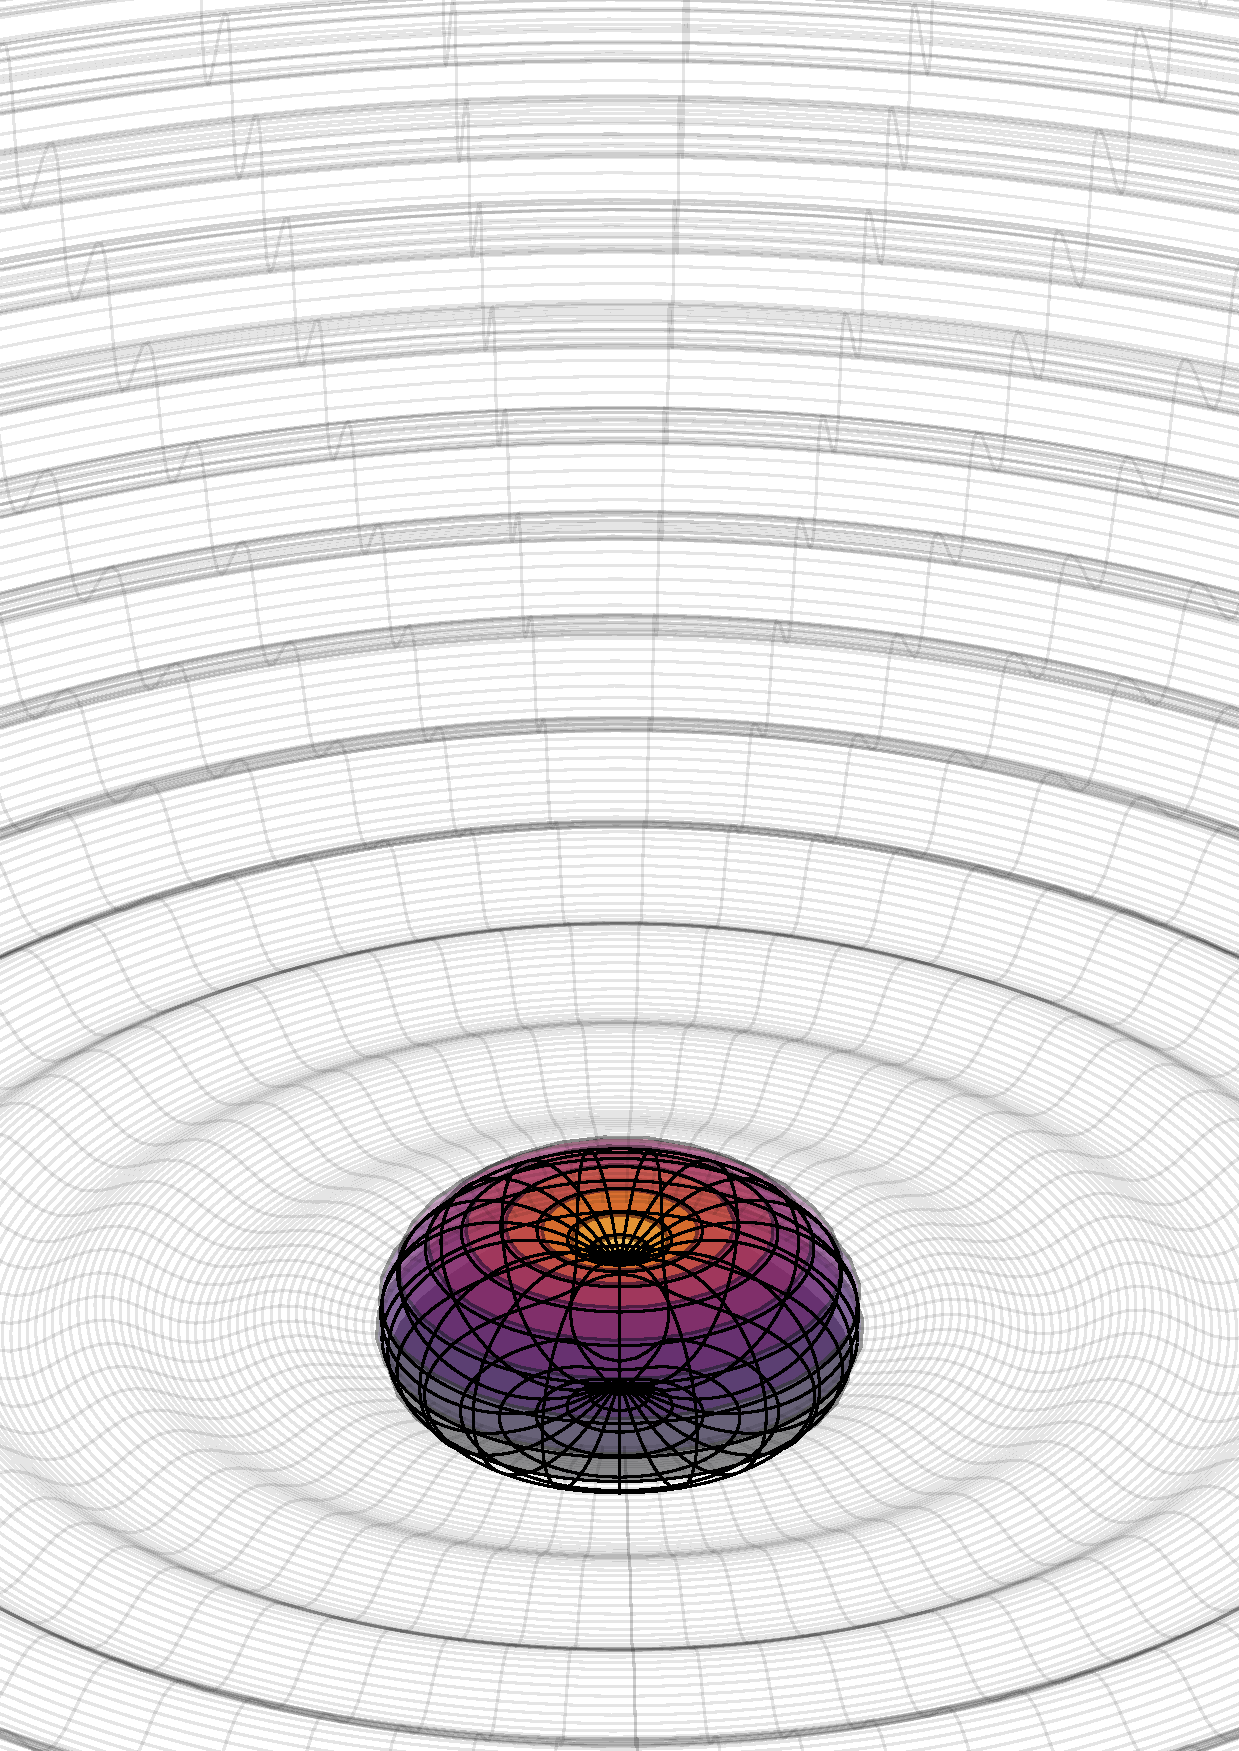
\includegraphics[width=\paperwidth, height=\paperheight]{figs/title2.pdf}};

\begin{center}
    \huge\fontfamily{phv}\selectfont\bfseries \mbox{X-ray bursts as a tool to} \mbox{constrain the equation of state} \mbox{of the ultra-dense matter} \mbox{inside neutron stars}

%\noindent\makebox[\linewidth]{\rule{\paperwidth}{2.4pt}}
\end{center}

\noindent\makebox[\linewidth]{\rule{\paperwidth}{0.4pt}}

\begin{center}
\LARGE\fontfamily{phv}\selectfont Joonas Nättilä
\end{center}

\vspace{7cm}

\fboxsep0pt
\colorbox{black}{\begin{minipage}{15cm}
\begin{center}

    \phantom{bla}

    \large\fontfamily{phv}\selectfont\mbox{\color{white}{Turun yliopiston julkaisuja - Annales Universitatis Turkuensis }}
    \footnotesize\fontfamily{phv}\selectfont\mbox{\color{white}{Sarja - ser. A I osa - tom. 570 $\vert$ Astronomica - Chemica - Physica - Mathematica $\vert$ Turku 2017}}

    \phantom{bla}
\end{center}
\end{minipage}}
    


\end{titlepage}

\restoregeometry
% --------------------------------------------------
\clearpage
\newpage


\setlength{\parindent}{0cm}
\section*{University of Turku}

Faculty of Mathematics and Natural Sciences

Department of Physics and Astronomy

\section*{Supervised by}

Prof. Juri Poutanen

Tuorla Observatory

University of Turku

Finland

\vspace{0.5cm}
Dr. Jari Kajava

Tuorla Observatory

University of Turku

Finland

\vspace{0.5cm}
Dr. Sergey Tsygankov

Tuorla Observatory

University of Turku

Finland


\section*{Reviewed by}

Prof. Frederick K. Lamb

Department of Physics 

University of Illinois at Urbana-Champaign

USA

\vspace{0.5cm}
Dr. Jean in 't Zand

SRON Netherlands Institute for Space Research 

Netherlands




\section*{Opponent}

Prof. Edward Brown

Department of Physics and Astronomy

Michigan State University

USA

\vspace{0.5cm}

The originality of this thesis has been checked in accordance with the University of Turku quality assurance system using the Turnitin OriginalityCheck service.

\vspace{0.5cm}

ISBN 978-951-29-7056-8 (PRINT) 

ISBN 978-951-29-7057-5 (PDF)

ISSN 0082-7002 (PRINT)

ISSN 2343-3175 (ONLINE) 

Painosalama Oy - Turku, Finland 2017


\setlength{\parindent}{1.5em}
